\documentclass[a4paper,14pt]{extarticle}

\usepackage[utf8x]{inputenc}
\usepackage[T1,T2A]{fontenc}
\usepackage[russian]{babel}
\usepackage{hyperref}
\usepackage{indentfirst}
\usepackage{here}
\usepackage{array}
\usepackage{graphicx}
\usepackage{caption}
\usepackage{subcaption}
\usepackage{chngcntr}
\usepackage{amsmath}
\usepackage{amssymb}
\usepackage{pgfplots}
\usepackage{pgfplotstable}
\usepackage[left=2cm,right=2cm,top=2cm,bottom=2cm,bindingoffset=0cm]{geometry}
\usepackage{multicol}
\usepackage{askmaps}
\usepackage{titlesec}
\usepackage{listings}
\usepackage{color}
\usepackage{courier}

\definecolor{green}{rgb}{0,0.6,0}
\definecolor{gray}{rgb}{0.5,0.5,0.5}
\definecolor{purple}{rgb}{0.58,0,0.82}

\lstset{
	language=Verilog,
	backgroundcolor=\color{white},   
	basicstyle=\small\ttfamily,
	commentstyle=\color{green},
	keywordstyle=\color{blue},	
	numberstyle=\tiny\color{gray},
	stringstyle=\color{purple},
	breakatwhitespace=false,
	breaklines=true,
	captionpos=b,
	keepspaces=true,
	numbers=left,
	numbersep=5pt,
	showspaces=false,
	showstringspaces=false,
	showtabs=false,
	tabsize=4,
	frame=single,
	inputpath={../quartus/},
	literate={~} {$\sim$}{1}
}

\renewcommand{\le}{\ensuremath{\leqslant}}
\renewcommand{\leq}{\ensuremath{\leqslant}}
\renewcommand{\ge}{\ensuremath{\geqslant}}
\renewcommand{\geq}{\ensuremath{\geqslant}}
\renewcommand{\epsilon}{\ensuremath{\varepsilon}}
\renewcommand{\phi}{\ensuremath{\varphi}}
\renewcommand{\thefigure}{\arabic{figure}} 	
\renewcommand*\not[1]{\overline{#1}}

\titleformat*{\section}{\large\bfseries} 
\titleformat*{\subsection}{\normalsize\bfseries} 
\titleformat*{\subsubsection}{\normalsize\bfseries} 
\titleformat*{\paragraph}{\normalsize\bfseries} 
\titleformat*{\subparagraph}{\normalsize\bfseries} 

\counterwithin{figure}{section}
\counterwithin{equation}{section}
\counterwithin{table}{section}
\newcommand{\sign}[1][5cm]{\makebox[#1]{\hrulefill}}
\graphicspath{{../pics/}}
\captionsetup{justification=centering,margin=1cm}
\def\arraystretch{1.3}
\setlength\parindent{5ex}
\titlelabel{\thetitle.\quad}

\begin{document}

\begin{titlepage}
\begin{center}
	Санкт-Петербургский Политехнический Университет Петра Великого\\[0.3cm]
	Институт компьютерных наук и технологий \\[0.3cm]
	Кафедра компьютерных систем и программных технологий\\[4cm]
	
	\textbf{ОТЧЕТ}\\ 
	\textbf{по лабораторной работе}\\[0.5cm]
	\textbf{SystemVerilog №4}\\[0.1cm]
	Автоматизация проектирования\\ дискретных устройств\\[4.0cm]
\end{center}

\begin{flushright}
	\begin{minipage}{0.45\textwidth}
		\textbf{Работу выполнил студент}\\[3mm]
		группа 33501/4 \hspace*{9mm} Дьячков В.В.\\[5mm]
		\textbf{Преподаватель}\\[5mm]
		\sign[1.5cm] \hspace*{1mm} к.т.н., доц. Филиппов А.С. \\[5mm]
	\end{minipage}
\end{flushright}

\vfill

\begin{center}
	Санкт-Петербург\\
	\the\year
\end{center}
\end{titlepage}

\addtocounter{page}{1}
\counterwithin{lstlisting}{section}

\section*{Используемые сокращения}
\addcontentsline{toc}{section}{Используемые сокращения}

\begin{itemize}
	\item FIFO -- First In First Out
	\item LVDS -- Low-Voltage Differencial Signaling
	\item PLL -- ФАПЧ (фазовая автоподстройка частоты)
	\item SDC -- Synopsys Design Constraints
\end{itemize}

\newpage

\section*{Задание на курсовое проектирование}
\addcontentsline{toc}{section}{Задание на курсовое проектирование}

\subsection*{Краткое описание}
\addcontentsline{toc}{subsection}{Краткое описание}

Устройство передачи данных решает три укрупненных задачи:
\begin{enumerate}
	\item Прием и буферизация данных от нескольких источников синхронных сигналов (синхросигнал расположен фронтом по центру бита, фазовый разброс $\pm1$ нс). Поток входных данных идет непрерывно.
	\item Когда в буфере FIFO накапливаются данные, достаточные для формирования пакета, устройство управления выдает команду блоку коммутации и формирования пакета, который формирует пакет в соответствии с заданием. Если данные для передачи отсутствуют, передается "пустой" пакет с отсутствующими данными, \code{M = 0} по каналу \code{N = 15}.
	\item LVDS Transmitter -- передатчик LVDS канала обеспечивает передачу синхронных дифференциальных данных по заданному числу каналов (Number of Channels) с заданной скоростью передачи (Output data rate).
\end{enumerate}

Укрупненная структурная схема устройства передачи данных.
\begin{figure}[H]
	\centering
	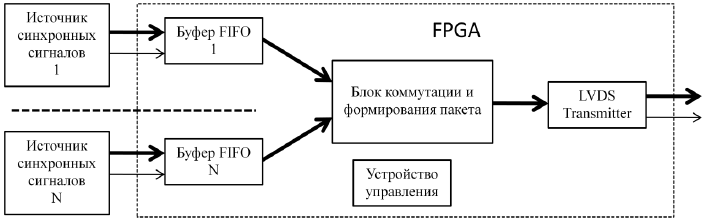
\includegraphics[width=\linewidth]{structure}
\end{figure}

\subsection*{Решаемые задачи}
\addcontentsline{toc}{subsection}{Решаемые задачи}

\begin{itemize}

	\item Анализ технического задания
	\begin{itemize}
		\item Анализ вариантов реализации и разработка структурной семы устройства.
		\item Детализация структурных блоков, разработка функциональной схемы устройства.
		\item Анализ IP-функций, используемых в устройстве, формирование требований к разрабатываемым блокам.
			\begin{itemize}
				\item[$\circ$] \code{FIFO}
				\item[$\circ$] \code{ALTLVDS_TX}\\[5mm]
			\end{itemize}
	\end{itemize}
	
	\item Разработка функционально-логического описания и моделирование
	\begin{itemize}
		\item Организация FIFO.
		\item Организация и настройка передатчика LVDS.
		\item Разработка блока коммутации.
		\item Разработка устройства управления.
		\item Интеграция разработанных блоков и моделирование работы устройства передачи данных.
	\end{itemize}
	
	
	\item Верификация устройства передачи данных в системном окружении
	\begin{itemize}
		\item Разработка имитатора системного окружения, задающего поток входных данных.
		\item Создание и настройка средств системной отладки.
		\item Исследование работы устройства передачи данных на плате-прототипе (Mini DiLab).
	\end{itemize}

\end{itemize}

\subsection*{Вариант индивидуального задания}
\addcontentsline{toc}{subsection}{Вариант индивидуального задания}

\begin{itemize}
	\item Три 16-разрядных источника сигналов, частота 10 МГц;
	\item Количество байт данных \code{M = 9};
	\item Формат пакета: <<\code{H1MD}>> (\code{H1} -- первый байт заголовка \code{0xFN}, где \code{N} -- номер канала; \code{M} -- количество байт данных; \code{D} -- передаваемые данные);
 	\item Двухканальный LVDS-передатчик, скорость передачи данных $600$ Мб/с.
\end{itemize}

\newpage

\section*{Введение}
\addcontentsline{toc}{section}{Введение}

Передача данных -- физический перенос данных (цифрового битового потока) в виде сигналов от точки к точке или от точки к нескольким точкам средствами электросвязи по каналу передачи данных. Обычно принятые данные обрабатываются средствами вычислительной техники. Примерами каналов передачи могут служить медные провода, волоконно-оптическая линия передачи, беспроводные каналы передачи данных или запоминающее устройство.

Передаваемые данные могут быть цифровыми сообщениями, идущими из источника данных, например, из компьютера или от клавиатуры. Это может быть и аналоговый сигнал — телефонный звонок или видеосигнал, оцифрованный в битовый поток, используя импульсно-кодирующую модуляцию (PCM) или более расширенные схемы кодирования источника (аналого-цифровое преобразование и сжатие данных). Кодирование источника и декодирование осуществляется кодеком или кодирующим оборудованием.

В проекте разрабатывается устройство передачи данных, принимающее данные с нескольких источников синхронных сигналов с непрерывным потоком. Разработанное устройство должно формировать пакеты для отправки их в канал связи с использование LVDS-передатчика.

\newpage

\tableofcontents

\newpage

\section{Разработка устройства передачи данных}

\subsection{Общая схема устройства}

На рис. \ref{fig:transmitter-scheme} приведена схема разрабатываемого устройства передачи данных. Устройство состоит из трех входных буферов, блока коммутации и LVDS-передатчика.
\begin{figure}[H]
	\centering
	\includegraphics[width=0.9\linewidth]{transmitter/scheme}
	\caption{Общая схема устройства передачи данных}
	\label{fig:transmitter-scheme}
\end{figure}

\subsection{Входной буфер}

На рис. \ref{fig:input-buffer-scheme} приведена схема входного буфера.
\begin{figure}[H]
	\centering
	\includegraphics[width=0.85\linewidth]{input_buffer/scheme}
	\caption{Схема входного буфера}
	\label{fig:input-buffer-scheme}
\end{figure}

Входной буфер накапливает входные данные при \code{write_req = 1} и, когда данных достаточно для формирования пакета (больше 9 байт), блок устанавливает флаг \code{input_ready = 1}. При \code{read_req = 1} буфер выдает накопленные данные. Блок состоит из блока FIFO, созданного на основе мегафункции \code{FIFO} (разрядность входа -- 16 бит, разрядность выхода -- 8 бит, глубина -- 64 слова) и компаратора для определения заполненности буфера. 

\newpage \noindent Блок содержит следующие входы и выходы:

\begin{itemize}
	\item Входы:
	\begin{itemize}
		\item \code{read_clk} -- тактовый сигнал чтения данных;
		\item \code{write_clk} -- тактовый сигнал записи данных;
		\item \code{arst} -- флаг асинхронного сброса;
		\item \code{read_req} -- разрешение на чтение данных;
		\item \code{write_req} -- разрешение на запись данных;
		\item \code{input_data[15:0]} -- входные данные.
	\end{itemize}
	\item Выходы:
	\begin{itemize}
		\item \code{input_ready} -- сигнал заполненности буфера;
		\item \code{output_data[7:0]} -- выходные данные. 
	\end{itemize}
\end{itemize}

\subsection{Блок коммутации и формирования пакета}

На рис. \ref{fig:commutator-scheme} приведена схема блока коммутации. 
\begin{figure}[H]
	\centering
	\includegraphics[width=0.95\linewidth]{commutator/scheme}
	\caption{Схема входного буфера}
	\label{fig:commutator-scheme}
\end{figure}

Блок коммутации и формирования пакета (коммутатор) принимает сигналы от трех входных буферов, формирует пакет и посылает его на LVDS-передатчик. 

Блок содержит следующие входы и выходы:

\begin{itemize}
	\item Входы:
	\begin{itemize}
		\item \code{clk} -- тактовый сигнал;
		\item \code{arst} -- флаг асинхронного сброса;
		\item \code{input_ready[2:0]} -- флаги готовности входных буферов к чтению;
		\item \code{input_data[23:0]} -- входные данные от трех буферов.
	\end{itemize}
	\item Выходы:
	\begin{itemize}
		\item \code{output_data[7:0]} -- выходные данные;
		\item \code{read_req[2:0]} -- сигналы запроса на чтение данных, подаваемые на входные буферы.
	\end{itemize}
\end{itemize}

\subsubsection{Шифратор номера канала}

Шифратор номера канала преобразует 3-разрядный код \code{pos[2:0]}, образуемый сигналами готовности трех входных буферов, в двоичный номер канала \code{bin[3:0]} и формирует соответствующий позиционный код с одной единицей \code{one_bit[2:0]}. 

Блок содержит следующие входы и выходы:

\begin{itemize}
	\item Входы:
	\begin{itemize}
		\item \code{clk} -- тактовый сигнал;
		\item \code{arst} -- флаг асинхронного сброса;
		\item \code{ena} -- разрешение на изменение номера активного канала;
		\item \code{bin[2:0]} -- сигналы готовности от входных буферов.
	\end{itemize}
	\item Выходы:
	\begin{itemize}
		\item \code{bin[3:0]} -- номер активного канала, используемый в заголовке пакета;
		\item \code{one_bit[2:0]} -- позиционный код активного канала.
	\end{itemize}
\end{itemize}

\subsubsection{Мультиплексор входных данных}

Мультиплексор выполняет коммутацию данных из трех входных буферов \code{input_data[23:0]} на выход блока \code{output_data[7:0]} для формирования пакета. В качестве кода управления используется номер канала \code{channel}, полученный от шифратора номера канала. 

Блок содержит следующие входы и выходы:

\begin{itemize}
	\item Входы:
	\begin{itemize}
		\item \code{clk} -- тактовый сигнал;
		\item \code{arst} -- флаг асинхронного сброса;
		\item \code{channel[3:0]} -- активный канал;
		\item \code{input_data[23:0]} -- данные от входных буферов.
	\end{itemize}
	\item Выходы:
	\begin{itemize}
		\item \code{output_data[7:0]} -- данные, считанные из активного канала.
	\end{itemize}
\end{itemize}

\subsubsection{Устройство управления}

Устройство управления согласует правильную работу устройств внутри коммутатора. После запуска устройства блок непрерывно формирует управляющий код данных \code{sel[1:0]} для отправки, который подается на мультиплексор выходных данных. При поступлении сигнала готовности входных данных \code{input_ready} формируется запрос на чтение из активного канала \code{read_req}. Блок содержит следующие входы и выходы:

\begin{itemize}
	\item Входы:
	\begin{itemize}
		\item \code{clk} -- тактовый сигнал;
		\item \code{arst} -- флаг асинхронного сброса;
		\item \code{input_ready} -- флаг готовности хотя бы одного буфера.
	\end{itemize}
	\item Выходы:
	\begin{itemize}
		\item \code{sel[1:0]} -- управляющий сигнал для мультиплексора выходных данных (\code{2'b00} -- заголовок, \code{2'b01} -- длина данных, \code{2'b10} -- данные); 
		\item \code{output_ready} -- сигнал, запрещающий шифратору номера канала изменять активный канал;
		\item \code{read_req} -- сигнал-запрос на чтение активного буфера, побитово умножается на \code{one_bit} шифратора канала и отправляется на входные буферы.
	\end{itemize}
\end{itemize}

\subsubsection{Мультиплексор выходных данных}

Мультиплексор определяет часть пакета, подаваемую на выход коммутатора. В зависимости от управляющего входа \code{sel[1:0]}, на выход может быть подан заголовок пакета \code{header[7:0]}, длина данных \code{length[7:0]} или данные с выхода буфера \code{data[7:0]}. Блок содержит следующие входы и выходы:

\begin{itemize}
	\item Входы:
	\begin{itemize}
		\item \code{clk} -- тактовый сигнал;
		\item \code{arst} -- флаг асинхронного сброса;
		\item \code{header[7:0]} -- байт заголовка;
		\item \code{length[7:0]} -- байт длины данных;
		\item \code{data[7:0]} -- байт данных.
	\end{itemize}
	\item Выход:
	\begin{itemize}
		\item \code{output_data[7:0]} -- выходные данные.
	\end{itemize}
\end{itemize}

\newpage

\subsection{LVDS-передатчик}

На рис. \ref{fig:lvds-transmitter-scheme} приведена схема блока LVDS-передатчика. 
\begin{figure}[H]
	\centering
	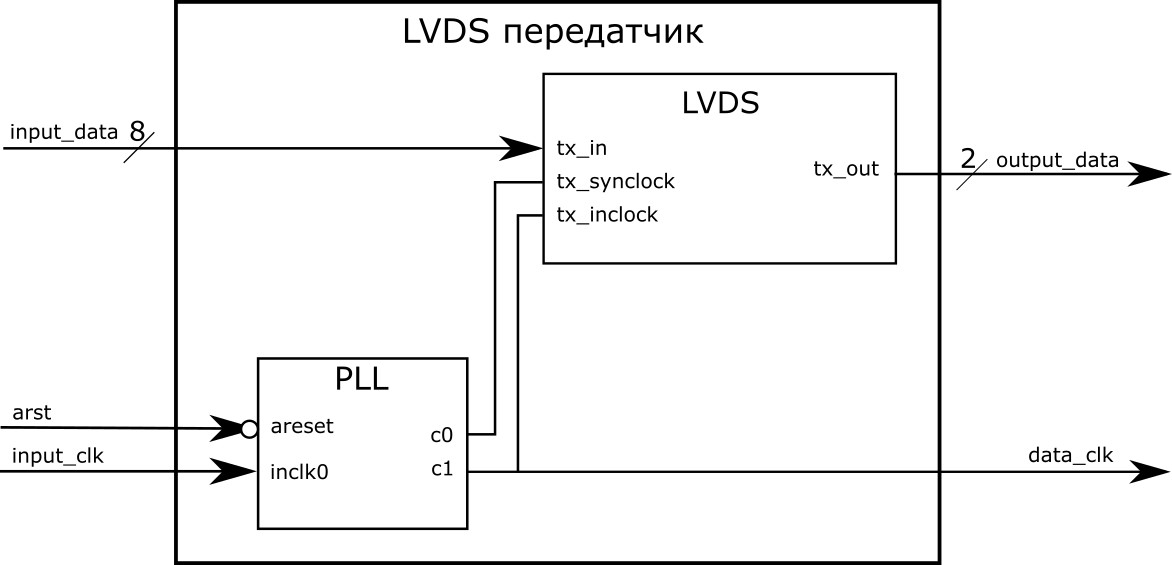
\includegraphics[width=0.9\linewidth]{lvds_transmitter/scheme}
	\caption{Схема LVDS-передатчика}
	\label{fig:lvds-transmitter-scheme}
\end{figure}

Блок состоит из делителя частоты PLL, созданного на основе мегафункции \code{ALTPLL} (входная частота -- 100 МГц, выходные частоты -- 150 МГц и 300 МГц), и LVDS-передатчика, созданного на основе мегафункции \code{ALTLVDS_TX} (количество каналов -- 2, фактор десериализации -- 4). 

Блок содержит следующие входы и выходы:

\begin{itemize}
	\item Входы:
		\begin{itemize}
			\item \code{input_clk} -- тактовый сигнал, поступающий на вход PLL;
			\item \code{arst} -- флаг асинхронного сброса;
			\item \code{input_data[7:0]} -- отправляемые данные.
		\end{itemize}
	\item Выходы:
		\begin{itemize}
			\item \code{data_clk} -- тактовый сигнал, используемый в блоке коммутации;
			\item \code{output_data[1:0]} -- данные, получаемые от LVDS-передатчика. 
		\end{itemize}
\end{itemize}

\subsection{Разработка временных требований}

Для передачи данных со скоростью 600 Мб/с, LVDS-передатчик должен получать два тактовых сигнала: быстрый с частотой 300 МГц ($\frac{\text{скорость передачи}}{2}$) и медленный с частотой 150 МГц ($\frac{\text{скорость передачи}}{\text{фактор десериализации}}$). Формирование 8-разрядных слов на выходе коммутатора должно осуществляться с частотой, равной медленной частоте LVDS-передатчика, то есть 150 МГц. Для получения нужных частот был использован PLL с входной частотой 100 МГц. Для задания соответствующих временных требований был создан SDC файл, приведенный в листинге \ref{code:sdc}.

\lstinputlisting[language=Tcl, caption=\code{transmitter.sdc}, label=code:sdc, morekeywords={create_clock, derive_clock_uncertainty}]{transmitter.sdc}

Созданный SDC файл был подключен к проекту, после чего проект был скомпилирован. Оставшееся предупреждение сообщает о невыполненом назначении контактов. На рис. \ref{fig:compile-report} приведен отчет компиляции.
\begin{figure}[H]
	\centering
	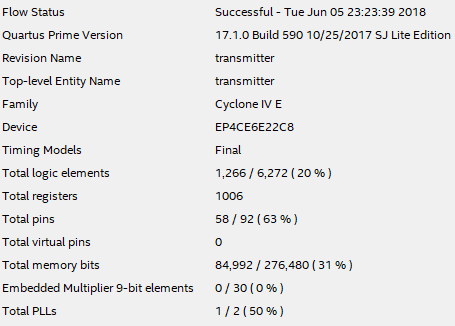
\includegraphics[scale=1]{compile/report}
	\caption{Отчет компиляции}
	\label{fig:compile-report}
\end{figure}

На рис. \ref{fig:compile-fmax} приведена информация о частоте работы проекта \code{Fmax}. Из отчета видно, что временные параметры, заданные в SDC файле, выполнены.
\begin{figure}[H]
	\centering
	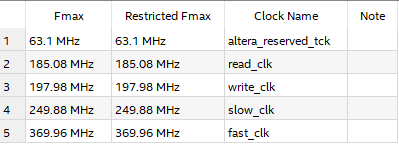
\includegraphics[scale=1]{compile/fmax}
	\caption{Частота работы проекта}
	\label{fig:compile-fmax}
\end{figure}

\section{Моделирование работы устройства}

\subsection{Буфер входных данных}

С помощью инструментов Quartus II было выполнено моделирование компонентов устройства и всего передатчика. На рис. \ref{fig:input_buffer_modelling} приведены результаты моделирования буфера входных данных. 
\begin{figure}[H]
	\centering
	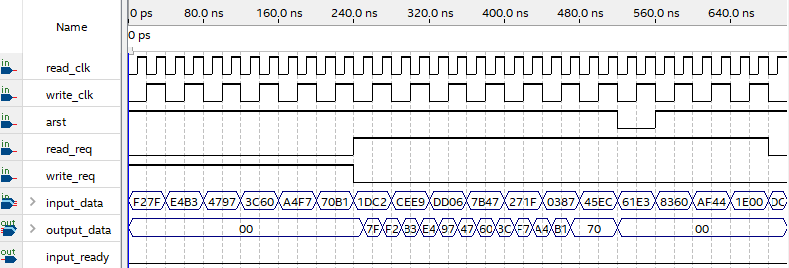
\includegraphics[width=\linewidth]{input_buffer/modelling}
	\caption{Результаты моделирования буфера входных данных}
	\label{fig:input_buffer_modelling}
\end{figure}

Из временной диаграммы видно, что на протяжении первых тактов \code{write_clk} выходные данные равны \code{0x00}, т.к. буфер накапливает минимально необходимые 9 байт для передачи по каналу: по 2 байта за одну запись. После чего устанавливается в единицу флаг \code{input_ready} и при \code{read_req = 1} начинает выдавать накопленные данные в порядке их получения.

\subsection{Блок коммутации и формирования пакета}

На рис. \ref{fig:commutator_modelling} приведены результаты моделирования блока коммутации.
\begin{figure}[H]
	\centering
	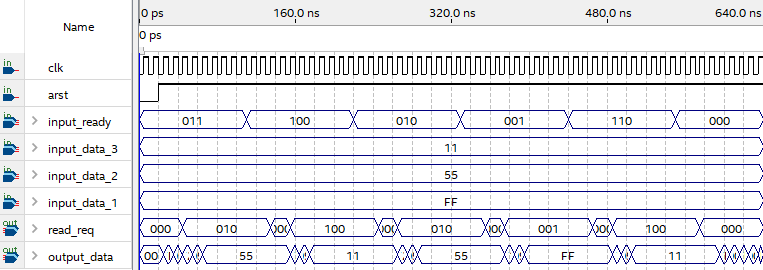
\includegraphics[width=\linewidth]{commutator/modelling}
	\caption{Результаты моделирования блока коммутации}
	\label{fig:commutator_modelling}
\end{figure}

Из временной диаграммы видно, что в зависимости от значения \code{input_ready} коммутатор формирует пакет из данных с одного из входных буферов, устанавливая в единицу соответствующий бит в \code{read_req}, или пустой пакет в случае отсутствия данных.

\subsubsection{Шифратор номера канала}

На рис. \ref{fig:channel_encoder_modelling} приведены результаты моделирования шифратора номера канала.
\begin{figure}[H]
	\centering
	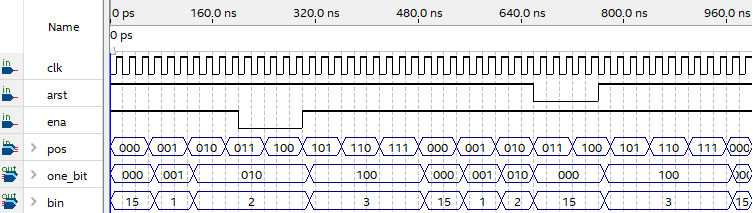
\includegraphics[width=\linewidth]{channel_encoder/modelling}
	\caption{Результаты моделирования шифратора номера канала}
	\label{fig:channel_encoder_modelling}
\end{figure}

\noindent Из временной диаграммы видно, что шифратор анализирует значение \code{pos[2:0]} и вычисляет номер активного канала, отдавая приоритет каналу с наибольшим номером. Если \code{pos = 3'b000}, то в соответствии с заданием выбирается канал \code{15}, а \code{one_bit = 3'b000}.

\subsubsection{Мультиплексор входных данных}

На рис. \ref{fig:input_muxer_modelling} приведены результаты моделирования мультиплексора входных данных.
\begin{figure}[H]
	\centering
	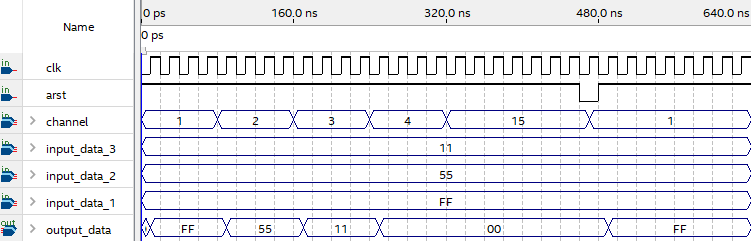
\includegraphics[width=\linewidth]{input_muxer/modelling}
	\caption{Результаты моделирования мультиплексора входных данных}
	\label{fig:input_muxer_modelling}
\end{figure}

Из временной диаграммы видно, что в зависимости от входного значения \code{channel[2:0]}, соответствующего номеру активного канала, мультиплексор передает на выход соответствующие 8 разрядов \code{input_data[23:0]}.

\subsubsection{Устройство управления}

На рис. \ref{fig:control_unit_modelling} приведены результаты моделирования устройства управления.
\begin{figure}[H]
	\centering
	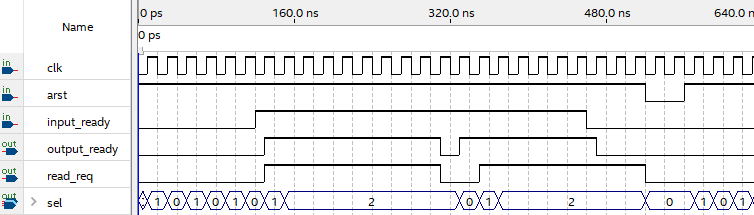
\includegraphics[width=\linewidth]{control_unit/modelling}
	\caption{Результаты моделирования устройства управления}
	\label{fig:control_unit_modelling}
\end{figure}

Из временной диаграммы видно, что в зависимости от флага \code{input_ready} устройство формирует последовательность управляющих воздействий для мультиплексора выходных данных. Так, когда \code{input_ready = 0} (ни один буфер не накопил нужного количества байт), формируется повторяющаяся последовательность \code{sel[1:0] = 0, 1, 0, 1...}, соответствующая передаче заголовка (\code{0xFF}) и длины данных (\code{0x00}). При \code{input_ready = 1} после отправки длины данных на 9 тактов состояние \code{sel[1:0] = 2}, что соответствует чтению из активного буфера.

\subsubsection{Мультиплексор выходных данных}

На рис. \ref{fig:output_muxer_modelling} приведены результаты моделирования мультиплексора выходных данных.
\begin{figure}[H]
	\centering
	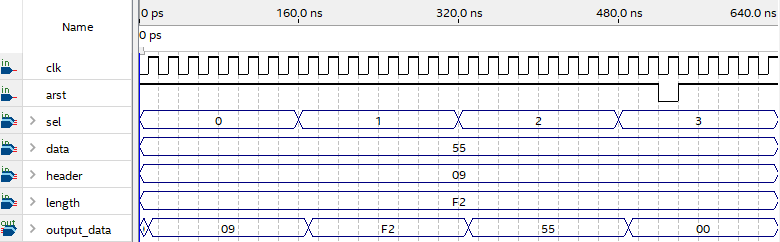
\includegraphics[width=\linewidth]{output_muxer/modelling}
	\caption{Результаты моделирования мультиплексора выходных данных}
	\label{fig:output_muxer_modelling}
\end{figure}

Из временной диаграммы видно, что в зависимости от значения управляющего кода \code{sel[1:0]} на выход передаются заголовок, длина сообщения или данные. Состояние \code{sel[1:0] = 3} ошибочно и не должно поступать на вход при правильной работе устройства управления.

\subsection{LVDS-передатчик}

На рис. \ref{fig:lvds_transmitter_modelling} приведены результаты моделирования LVDS-передатчика.
\begin{figure}[H]
	\centering
	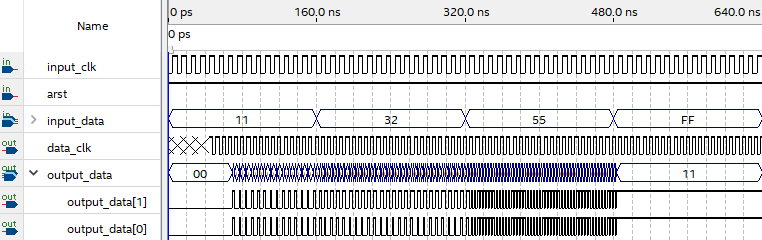
\includegraphics[width=\linewidth]{lvds_transmitter/modelling}
	\caption{Результаты моделирования LVDS-передатчика}
	\label{fig:lvds_transmitter_modelling}
\end{figure}

Из временной диаграммы видно, что передатчик преобразует входящие данные \code{input_data[7:0]} в \code{output_data[1:0]}, получаемые из двухканального LVDS-передатчика.

\subsection{Устройство передачи данных}

На рис. \ref{fig:transmitter_modelling} приведены результаты моделирования устройства передачи данных.
\begin{figure}[H]
	\centering
	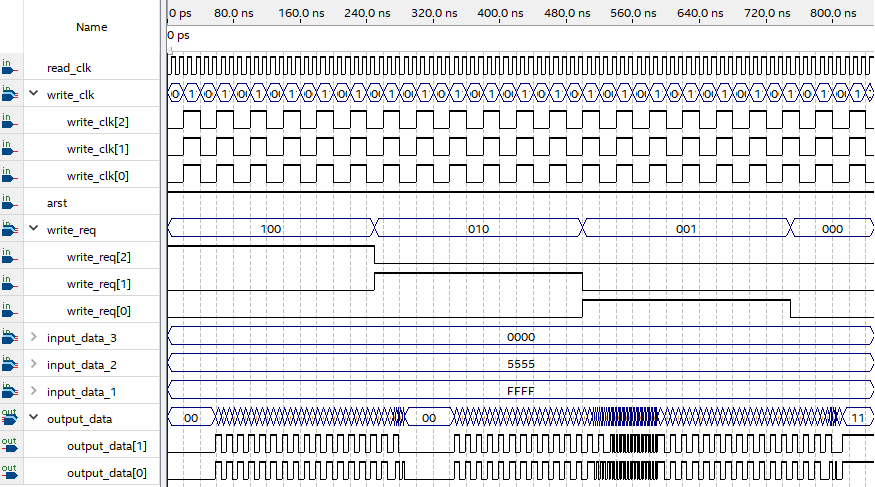
\includegraphics[width=\linewidth]{transmitter/modelling}
	\caption{Результаты моделирования устройства передачи данных}
	\label{fig:transmitter_modelling}
\end{figure}

Из временной диаграммы видно, что три буфера поочередно заполняются при помощью разрешения на запись \code{write_req[2:0]}, после чего соответствующие значения поступают на выход с LVDS-передатчика \code{output_data[1:0]}. На 280--330~нс передается значение \code{0x0000}, на 500--540 нс передается шахматный код \code{0x5555}, а после 840 нс передается \code{0xFFFF}. Между этими тремя передачами происходит передача пустых пакетов (номер канала \code{0xFF}, длина данных \code{0x00}), так как частота \code{read_clk} значительно выше, чем \code{write_clk}.

\section{Проверка работы устройства на плате}

Для проверки работы устройства было создано описание, использующее PLL (для настройки тактовой частоты) и разработанный передатчик. Значение с переключателей \code{sw[7:0]} интерпретируется как входные данные, кнопка \code{pba} используется для асинхронного сброса, кнопка \code{pbb} задает номер буфера, в который можно записывать данные. Выходы передатчика подключены к диодам \code{led[1:0]}.

После программирования платы был подключен статический анализатор SignalTap II. С его помощью был выполнен контроль внутреннего состояния разработанного устройства. Для контроля были выбраны тактовые сигналы чтения \code{read_clk} и записи \code{write_clk}, сигнал асинхронного сброса \code{arst = pba}, разрешение буферов на запись данных \code{write_req[2:0] = pbb ? 3'b100 : 3'b001}, данные на входе \code{data[47:0] = \{sw + 8'd1, sw + 8'd1, sw, sw, sw - 8'd1, sw - 8'd1\}} и формируемые коммутатором пакеты \code{out}. В качестве события для срабатывания захвата данных было задано изменение состояния \code{pbb}. На рис. \ref{fig:dilab_modelling} изображены результаты проверки работы устройства на плате.

\begin{figure}[H]
	\centering
	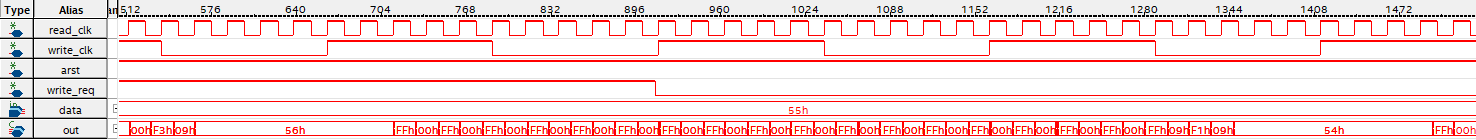
\includegraphics[width=\linewidth]{dilab/modelling_1}
	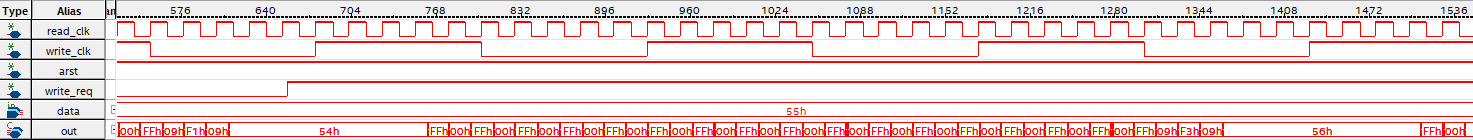
\includegraphics[width=\linewidth]{dilab/modelling_2}
	\caption{Результаты проверки работы устройства на плате}
	\label{fig:dilab_modelling}
\end{figure}

При \code{write_req = 1} на вход передатчика подается значение \code{0x56}, что соответствует входным данным на третьем канале (\code{sw + 8'd1}), а при \code{write_req = 0} подается значение \code{0x54}, что соответствует данным на первом канале (\code{sw - 8'd1}). Так как тактовая частота чтения выше, чем частота записи данных, между пакетами с данными отправляется большое количество пустых пакетов (\code{0xFF00}). Из диаграмм видно, что пакеты формируются верно: в заголовке указывается правильный источник данных, длина пакета и данные соответствуют передаваемым данным. Таким образом, устройство работает верно.

\newpage

\section*{Заключение}
\addcontentsline{toc}{section}{Заключение}

В процессе курсового проекта разработано устройство передачи данных и создано его функциональное описание на языке Verilog. Устройство решает следующие задачи: прием и буферизация данных от трех источников сигналов; формирование пакета, включающего заголовок, длину данных и передаваемые данные; передача сигналов по двум каналам с помощью LVDS-передатчика. Все блоки интегрированы в конечное устройство передатчика. 

Для устройства были заданы временные требования, для каждого блока разработанного устройства было выполнено функциональное моделирование. Работа устройства была проверена на плате с помощью статического анализатора SignalTap II. В результате выполнения работы удалось закрепить навыки работы с языком описания Verilog и получить опыт проектирования иерархического устройства, имеющего сложную структуру, а также закрепить навыки отладки устройств на плате.

\newpage

\section*{Список используемой литературы}
\addcontentsline{toc}{section}{Список используемой литературы}

\begin{enumerate}
	\item FIFO Intel ®FPGA IP User Guide // [Электронный ресурс.] --\\
	URL: \href{https://www.altera.com/en_US/pdfs/literature/ug/ug_fifo.pdf}{https://www.altera.com/en\_US/pdfs/literature/ug/ug\_fifo.pdf}\\
	(дата обращения: 01.06.2018)
	\item LVDS SERDES Transmitter / Receiver IP Cores User Guide // [Электронный ресурс.] --\\
	URL: \href{https://www.altera.com/en_US/pdfs/literature/ug/ug_altlvds.pdf}{https://www.altera.com/en\_US/pdfs/literature/ug/ug\_altlvds.pdf}\\
	(дата обращения: 02.06.2018)
	\item Altera Phase-Locked Loop (Altera PLL) IP Core User Guide // [Электронный ресурс.] --\\
	URL: \href{https://www.altera.com/en_US/pdfs/literature/ug/altera_pll.pdf}{https://www.altera.com/en\_US/pdfs/literature/ug/altera\_pll.pdf}\\
	(дата обращения: 03.06.2018)
\end{enumerate}

\newpage

\section*{Приложение. Исходный код на языке Verilog}
\addcontentsline{toc}{section}{Приложение. Исходный код на языке Verilog}

\subsection*{Буфер входных данных}

\lstinputlisting[caption=\code{input_buffer.v}]{input_buffer.v}

\subsection*{Блок коммутации и формирования пакета}

\lstinputlisting[caption=\code{commutator.v}]{commutator.v}

\newpage

\subsection*{Шифратор номера канала}

\lstinputlisting[caption=\code{channel_encoder.v}]{channel_encoder.v}

\subsection*{Мультиплексор входных данных}

\lstinputlisting[caption=\code{input_muxer.v}]{input_muxer.v}

\subsection*{Устройство управления}

\lstinputlisting[caption=\code{control_unit.v}]{control_unit.v}

\subsection*{Мультиплексор выходных данных}

\lstinputlisting[caption=\code{output_muxer.v}]{output_muxer.v}

\newpage

\subsection*{LVDS-передатчик}

\lstinputlisting[caption=\code{output_buffer.v}]{lvds_transmitter.v}

\subsection*{Устройство передачи данных}

\lstinputlisting[caption=\code{transmitter.v}]{transmitter.v}

\subsection*{Тестирование устройства на плате}

\lstinputlisting[caption=\code{transmitter_dilab.v}]{transmitter_dilab.v}

\end{document}